% Appendix E figure of "Galashin's Conjecture 4.3 via a convex gradient": the four cases of Lemma 20 on actual windows.
% Source in the paper's own fonts at the text width (6.5in). It adds no assertion and is used in no proof.
% Every value drawn is read from Lean output lines (SHA-256 of the lines), evaluated by the formal definitions of
% Conj43.WindowLemmas (the window, its residue permutation, the adjacent active ascent, the lift S, the edge sets):
%   picture D146 24b3645167e47b9352568863ef17d0828f87d80ffdbde611b8737af998c71674   (left, w = (4, 5, 6, 7))
%   picture D147 ec2782301f5f84f28ab305e5219a573f1cc78e2684249dd3f1253e926b54ef4b   (triangle, w = (3, 4, 5))
%   picture D148 ad56f236c337f1bb194197ff4356d8cc04cc36afa6f8bfbdb4b133f8b3d42d69   (right, w = (3, 4, 5, 6))
%   picture D145 7ec859ab47a8196e37cd8d6bbfa3e9bcbaf434c2a5de262d346f3b2606fdc69f   (A = b, w = (1, 3, 5))
% Build: pdflatex <this file> && pdftocairo -svg <this file>.pdf <this file>.svg
\documentclass[11pt]{standalone}
\usepackage[T1]{fontenc}
\usepackage{lmodern}
\usepackage{amsmath,amssymb}
\usepackage{tikz}
\usetikzlibrary{arrows.meta}
% the palette of the paper's other figures (Okabe-Ito): blue solid for alpha, ochre dashed for beta; bluish green and
% vermillion for the crossings the swap adds and removes
\definecolor{ink}{HTML}{233740}
\definecolor{muted}{HTML}{65757D}
\definecolor{pblue}{HTML}{0072B2}
\definecolor{qochre}{HTML}{B87827}
\definecolor{addg}{HTML}{009E73}
\definecolor{remv}{HTML}{D55E00}
\tikzset{
  base/.style={draw=muted, line width=0.5pt},
  exit/.style={circle, draw=ink, fill=white, line width=0.6pt, inner sep=0pt, minimum size=4.2pt},
  entry/.style={circle, draw=ink, fill=ink, line width=0.6pt, inner sep=0pt, minimum size=4.2pt},
  chA/.style={pblue, line width=1.1pt, -{Stealth[length=5pt,width=4.2pt]}, shorten >=2.2pt},
  chB/.style={qochre, line width=1.1pt, dash pattern=on 4pt off 1.6pt, -{Stealth[length=5pt,width=4.2pt]}, shorten >=2.2pt},
  chb/.style={ink, line width=1.1pt, -{Stealth[length=5pt,width=4.2pt]}, shorten >=2.2pt},
  chr/.style={muted, line width=0.7pt, -{Stealth[length=3.5pt,width=3pt]}, shorten >=2.2pt},
  added/.style={circle, draw=addg, fill=addg, inner sep=0pt, minimum size=5pt},
  removed/.style={rectangle, draw=remv, fill=remv, inner sep=0pt, minimum size=4.6pt},
  lab/.style={font=\footnotesize, inner sep=1.2pt, text=ink},
  rtitle/.style={font=\small, text=ink, inner sep=0pt, anchor=west},
  fnote/.style={font=\footnotesize, text=ink, inner sep=0pt, anchor=west},
}
\begin{document}
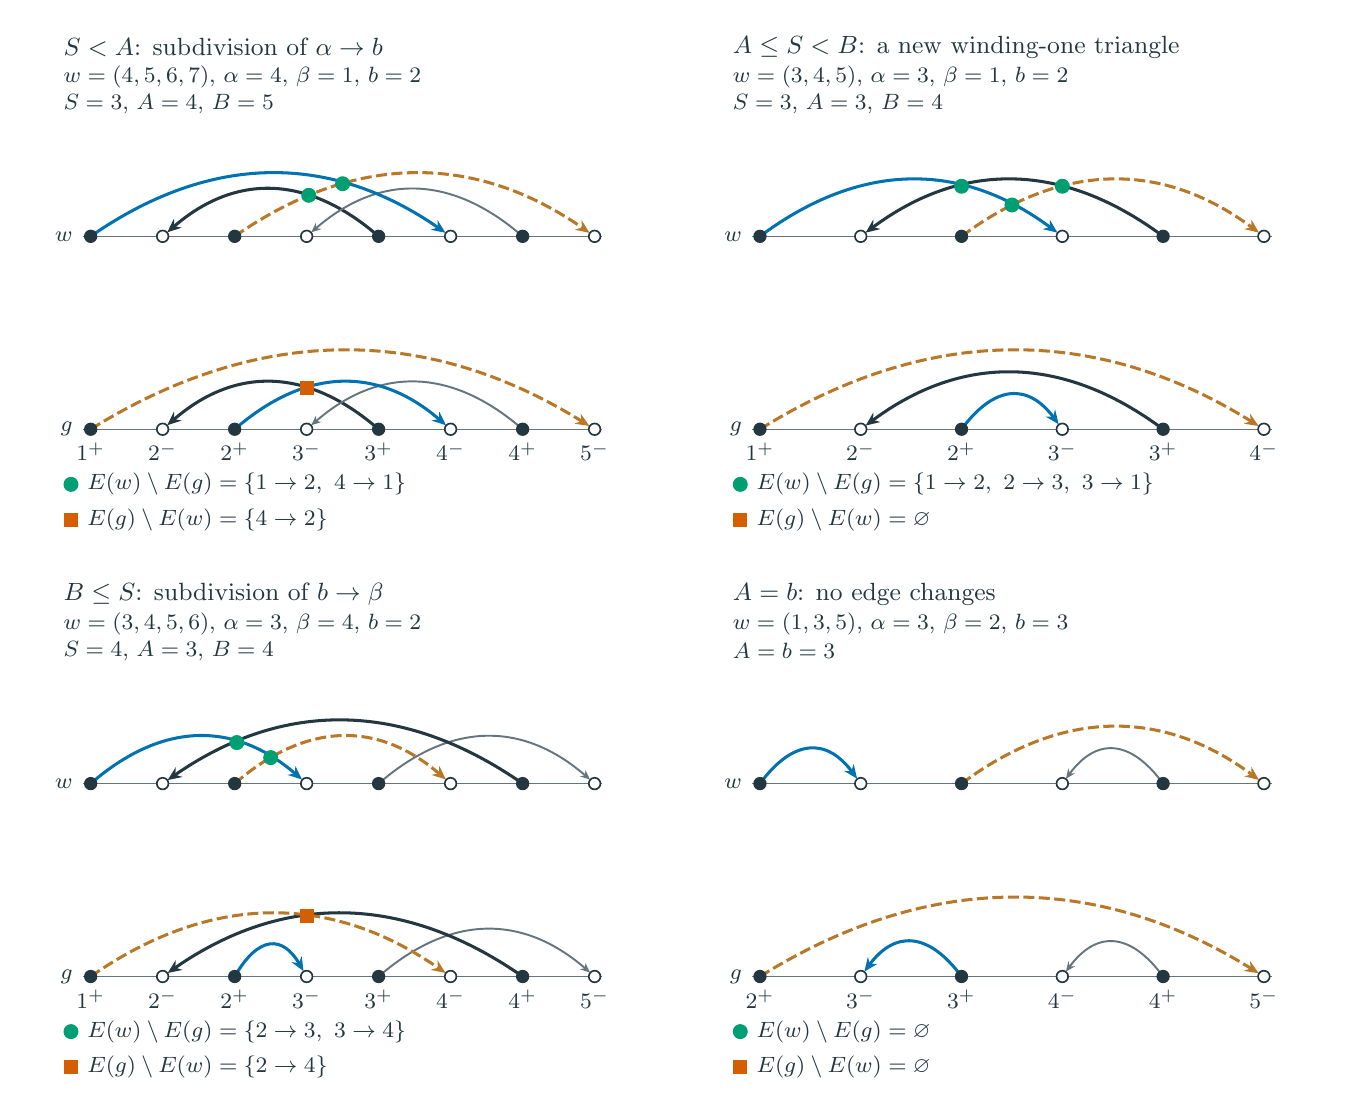
\begin{tikzpicture}[x=1cm,y=1cm]
\useasboundingbox (-0.25,-10.85) rectangle (16.26,2.65);
\node[rtitle] at (0.200,2.400) {$S<A$: subdivision of $\alpha\to b$};
\node[fnote] at (0.200,2.030) {$w=(4, 5, 6, 7)$, $\alpha=4$, $\beta=1$, $b=2$};
\node[fnote] at (0.200,1.680) {$S=3$, $A=4$, $B=5$};
\draw[base] (0.450,-0.000) -- (7.050,-0.000);
\node[lab, anchor=east] at (0.370,-0.000) {$w$};
\draw[chB] (2.379,-0.000) .. controls (3.902,1.061) and (5.426,1.061) .. (6.950,-0.000);
\draw[chb] (4.207,-0.000) .. controls (3.293,0.793) and (2.379,0.793) .. (1.464,-0.000);
\draw[chr] (6.036,-0.000) .. controls (5.121,0.793) and (4.207,0.793) .. (3.293,-0.000);
\draw[chA] (0.550,-0.000) .. controls (2.074,1.061) and (3.598,1.061) .. (5.121,-0.000);
\node[entry] at (0.550,-0.000) {};
\node[exit] at (1.464,-0.000) {};
\node[entry] at (2.379,-0.000) {};
\node[exit] at (3.293,-0.000) {};
\node[entry] at (4.207,-0.000) {};
\node[exit] at (5.121,-0.000) {};
\node[entry] at (6.036,-0.000) {};
\node[exit] at (6.950,-0.000) {};
\node[added] at (3.320,0.521) {};
\node[added] at (3.750,0.668) {};
\draw[base] (0.450,-2.450) -- (7.050,-2.450);
\node[lab, anchor=east] at (0.370,-2.450) {$g$};
\draw[chB] (0.550,-2.450) .. controls (2.683,-1.121) and (4.817,-1.121) .. (6.950,-2.450);
\draw[chb] (4.207,-2.450) .. controls (3.293,-1.657) and (2.379,-1.657) .. (1.464,-2.450);
\draw[chr] (6.036,-2.450) .. controls (5.121,-1.657) and (4.207,-1.657) .. (3.293,-2.450);
\draw[chA] (2.379,-2.450) .. controls (3.293,-1.657) and (4.207,-1.657) .. (5.121,-2.450);
\node[entry] at (0.550,-2.450) {};
\node[lab, anchor=north] at (0.550,-2.570) {$1^{+}$};
\node[exit] at (1.464,-2.450) {};
\node[lab, anchor=north] at (1.464,-2.570) {$2^{-}$};
\node[entry] at (2.379,-2.450) {};
\node[lab, anchor=north] at (2.379,-2.570) {$2^{+}$};
\node[exit] at (3.293,-2.450) {};
\node[lab, anchor=north] at (3.293,-2.570) {$3^{-}$};
\node[entry] at (4.207,-2.450) {};
\node[lab, anchor=north] at (4.207,-2.570) {$3^{+}$};
\node[exit] at (5.121,-2.450) {};
\node[lab, anchor=north] at (5.121,-2.570) {$4^{-}$};
\node[entry] at (6.036,-2.450) {};
\node[lab, anchor=north] at (6.036,-2.570) {$4^{+}$};
\node[exit] at (6.950,-2.450) {};
\node[lab, anchor=north] at (6.950,-2.570) {$5^{-}$};
\node[removed] at (3.293,-1.921) {};
\node[added] at (0.300,-3.150) {};
\node[fnote] at (0.500,-3.150) {$E(w)\setminus E(g)=\{1\to 2,\  4\to 1\}$};
\node[removed] at (0.300,-3.600) {};
\node[fnote] at (0.500,-3.600) {$E(g)\setminus E(w)=\{4\to 2\}$};
\node[rtitle] at (8.700,2.400) {$A\le S<B$: a new winding-one triangle};
\node[fnote] at (8.700,2.030) {$w=(3, 4, 5)$, $\alpha=3$, $\beta=1$, $b=2$};
\node[fnote] at (8.700,1.680) {$S=3$, $A=3$, $B=4$};
\draw[base] (8.950,-0.000) -- (15.550,-0.000);
\node[lab, anchor=east] at (8.870,-0.000) {$w$};
\draw[chB] (11.610,-0.000) .. controls (12.890,0.954) and (14.170,0.954) .. (15.450,-0.000);
\draw[chb] (14.170,-0.000) .. controls (12.890,0.954) and (11.610,0.954) .. (10.330,-0.000);
\draw[chA] (9.050,-0.000) .. controls (10.330,0.954) and (11.610,0.954) .. (12.890,-0.000);
\node[entry] at (9.050,-0.000) {};
\node[exit] at (10.330,-0.000) {};
\node[entry] at (11.610,-0.000) {};
\node[exit] at (12.890,-0.000) {};
\node[entry] at (14.170,-0.000) {};
\node[exit] at (15.450,-0.000) {};
\node[added] at (12.890,0.636) {};
\node[added] at (11.610,0.636) {};
\node[added] at (12.250,0.398) {};
\draw[base] (8.950,-2.450) -- (15.550,-2.450);
\node[lab, anchor=east] at (8.870,-2.450) {$g$};
\draw[chB] (9.050,-2.450) .. controls (11.183,-1.121) and (13.317,-1.121) .. (15.450,-2.450);
\draw[chb] (14.170,-2.450) .. controls (12.890,-1.496) and (11.610,-1.496) .. (10.330,-2.450);
\draw[chA] (11.610,-2.450) .. controls (12.037,-1.872) and (12.463,-1.872) .. (12.890,-2.450);
\node[entry] at (9.050,-2.450) {};
\node[lab, anchor=north] at (9.050,-2.570) {$1^{+}$};
\node[exit] at (10.330,-2.450) {};
\node[lab, anchor=north] at (10.330,-2.570) {$2^{-}$};
\node[entry] at (11.610,-2.450) {};
\node[lab, anchor=north] at (11.610,-2.570) {$2^{+}$};
\node[exit] at (12.890,-2.450) {};
\node[lab, anchor=north] at (12.890,-2.570) {$3^{-}$};
\node[entry] at (14.170,-2.450) {};
\node[lab, anchor=north] at (14.170,-2.570) {$3^{+}$};
\node[exit] at (15.450,-2.450) {};
\node[lab, anchor=north] at (15.450,-2.570) {$4^{-}$};
\node[added] at (8.800,-3.150) {};
\node[fnote] at (9.000,-3.150) {$E(w)\setminus E(g)=\{1\to 2,\  2\to 3,\  3\to 1\}$};
\node[removed] at (8.800,-3.600) {};
\node[fnote] at (9.000,-3.600) {$E(g)\setminus E(w)=\varnothing$};
\node[rtitle] at (0.200,-4.550) {$B\le S$: subdivision of $b\to\beta$};
\node[fnote] at (0.200,-4.920) {$w=(3, 4, 5, 6)$, $\alpha=3$, $\beta=4$, $b=2$};
\node[fnote] at (0.200,-5.270) {$S=4$, $A=3$, $B=4$};
\draw[base] (0.450,-6.950) -- (7.050,-6.950);
\node[lab, anchor=east] at (0.370,-6.950) {$w$};
\draw[chr] (4.207,-6.950) .. controls (5.121,-6.157) and (6.036,-6.157) .. (6.950,-6.950);
\draw[chb] (6.036,-6.950) .. controls (4.512,-5.889) and (2.988,-5.889) .. (1.464,-6.950);
\draw[chA] (0.550,-6.950) .. controls (1.464,-6.157) and (2.379,-6.157) .. (3.293,-6.950);
\draw[chB] (2.379,-6.950) .. controls (3.293,-6.157) and (4.207,-6.157) .. (5.121,-6.950);
\node[entry] at (0.550,-6.950) {};
\node[exit] at (1.464,-6.950) {};
\node[entry] at (2.379,-6.950) {};
\node[exit] at (3.293,-6.950) {};
\node[entry] at (4.207,-6.950) {};
\node[exit] at (5.121,-6.950) {};
\node[entry] at (6.036,-6.950) {};
\node[exit] at (6.950,-6.950) {};
\node[added] at (2.406,-6.429) {};
\node[added] at (2.836,-6.620) {};
\draw[base] (0.450,-9.400) -- (7.050,-9.400);
\node[lab, anchor=east] at (0.370,-9.400) {$g$};
\draw[chr] (4.207,-9.400) .. controls (5.121,-8.607) and (6.036,-8.607) .. (6.950,-9.400);
\draw[chb] (6.036,-9.400) .. controls (4.512,-8.339) and (2.988,-8.339) .. (1.464,-9.400);
\draw[chA] (2.379,-9.400) .. controls (2.683,-8.875) and (2.988,-8.875) .. (3.293,-9.400);
\draw[chB] (0.550,-9.400) .. controls (2.074,-8.339) and (3.598,-8.339) .. (5.121,-9.400);
\node[entry] at (0.550,-9.400) {};
\node[lab, anchor=north] at (0.550,-9.520) {$1^{+}$};
\node[exit] at (1.464,-9.400) {};
\node[lab, anchor=north] at (1.464,-9.520) {$2^{-}$};
\node[entry] at (2.379,-9.400) {};
\node[lab, anchor=north] at (2.379,-9.520) {$2^{+}$};
\node[exit] at (3.293,-9.400) {};
\node[lab, anchor=north] at (3.293,-9.520) {$3^{-}$};
\node[entry] at (4.207,-9.400) {};
\node[lab, anchor=north] at (4.207,-9.520) {$3^{+}$};
\node[exit] at (5.121,-9.400) {};
\node[lab, anchor=north] at (5.121,-9.520) {$4^{-}$};
\node[entry] at (6.036,-9.400) {};
\node[lab, anchor=north] at (6.036,-9.520) {$4^{+}$};
\node[exit] at (6.950,-9.400) {};
\node[lab, anchor=north] at (6.950,-9.520) {$5^{-}$};
\node[removed] at (3.293,-8.636) {};
\node[added] at (0.300,-10.100) {};
\node[fnote] at (0.500,-10.100) {$E(w)\setminus E(g)=\{2\to 3,\  3\to 4\}$};
\node[removed] at (0.300,-10.550) {};
\node[fnote] at (0.500,-10.550) {$E(g)\setminus E(w)=\{2\to 4\}$};
\node[rtitle] at (8.700,-4.550) {$A=b$: no edge changes};
\node[fnote] at (8.700,-4.920) {$w=(1, 3, 5)$, $\alpha=3$, $\beta=2$, $b=3$};
\node[fnote] at (8.700,-5.270) {$A=b=3$};
\draw[base] (8.950,-6.950) -- (15.550,-6.950);
\node[lab, anchor=east] at (8.870,-6.950) {$w$};
\draw[chr] (14.170,-6.950) .. controls (13.743,-6.372) and (13.317,-6.372) .. (12.890,-6.950);
\draw[chB] (11.610,-6.950) .. controls (12.890,-5.996) and (14.170,-5.996) .. (15.450,-6.950);
\draw[chA] (9.050,-6.950) .. controls (9.477,-6.372) and (9.903,-6.372) .. (10.330,-6.950);
\node[entry] at (9.050,-6.950) {};
\node[exit] at (10.330,-6.950) {};
\node[entry] at (11.610,-6.950) {};
\node[exit] at (12.890,-6.950) {};
\node[entry] at (14.170,-6.950) {};
\node[exit] at (15.450,-6.950) {};
\draw[base] (8.950,-9.400) -- (15.550,-9.400);
\node[lab, anchor=east] at (8.870,-9.400) {$g$};
\draw[chr] (14.170,-9.400) .. controls (13.743,-8.822) and (13.317,-8.822) .. (12.890,-9.400);
\draw[chB] (9.050,-9.400) .. controls (11.183,-8.071) and (13.317,-8.071) .. (15.450,-9.400);
\draw[chA] (11.610,-9.400) .. controls (11.183,-8.822) and (10.757,-8.822) .. (10.330,-9.400);
\node[entry] at (9.050,-9.400) {};
\node[lab, anchor=north] at (9.050,-9.520) {$2^{+}$};
\node[exit] at (10.330,-9.400) {};
\node[lab, anchor=north] at (10.330,-9.520) {$3^{-}$};
\node[entry] at (11.610,-9.400) {};
\node[lab, anchor=north] at (11.610,-9.520) {$3^{+}$};
\node[exit] at (12.890,-9.400) {};
\node[lab, anchor=north] at (12.890,-9.520) {$4^{-}$};
\node[entry] at (14.170,-9.400) {};
\node[lab, anchor=north] at (14.170,-9.520) {$4^{+}$};
\node[exit] at (15.450,-9.400) {};
\node[lab, anchor=north] at (15.450,-9.520) {$5^{-}$};
\node[added] at (8.800,-10.100) {};
\node[fnote] at (9.000,-10.100) {$E(w)\setminus E(g)=\varnothing$};
\node[removed] at (8.800,-10.550) {};
\node[fnote] at (9.000,-10.550) {$E(g)\setminus E(w)=\varnothing$};
\end{tikzpicture}
\end{document}
